%%%%%%%%%%%%%%%%%%%%%%%%%%%%%%%%%%%%%%%%%%%%%%%%%%%%%%%%%%%%%%%%%%%%%%
% Lớp 11 | Lý thuyết đồ thị | Đồ thị
% Dạng 1C2?1-2: Câu hỏi về bậc của đồ thị
% Số câu: 2  (sinh tự động bởi tach_cau.py; từ nay thầy sửa trực tiếp file này)
%%%%%%%%%%%%%%%%%%%%%%%%%%%%%%%%%%%%%%%%%%%%%%%%%%%%%%%%%%%%%%%%%%%%%%

%%%%%%%%%%%%%%%% TỰ LUẬN %%%%%%%%%%%%%%%%

% nguồn: Ok_TuanLuan_Toan11_Lan1
\begin{bt}%[1C2Y1-2]%[ma:eac7830e]
	Viết năm  số hạng đầu của mỗi dãy số có số hạng tổng quát $u_n$ cho bởi công thức sau:
	\begin{enumEX}{2}
		\item  $u_n = 2n^2 + 1$.
		\item  $u_n = \dfrac{(-1)^n}{2n-1}$.
		 \item $u_n = \dfrac{2^n}{n}$.
		\item  $u_n = \left( 1+\dfrac{1}{n} \right)^n$.
	\end{enumEX}
	 \loigiai{
		\begin{enumEX}{1}
			 \item Năm số hạng đầu của dãy số là
			 \[
			u_1 = 3;\ u_2  =9;\ u_3 = 19;\ u_4 = 33;\ u_5 = 51.
			 \]
			\item Năm số hạng đầu của dãy  số là
			\[ 
			u_1 = -1;\ u_2 =\dfrac{1}{3};\ u_3 = -\dfrac{1}{5};\ u_4 = \dfrac{1}{7};\  u_5 = -\dfrac{1}{9}.
			 \]
			\item Năm số  hạng đầu của dãy số là
			\[ 
			u_1 = 2;\ u_2 =2;\ u_3 = \dfrac{8}{3};\ u_4 = 4;\ u_5 =  \dfrac{32}{5}.
			 \]
			\item Năm số hạng  đầu của dãy số là
			 \[
			u_1 =  2;\ u_2 =\dfrac{9}{4};\ u_3 = \dfrac{64}{27};\ u_4 = \dfrac{625}{256};\ u_5 = \dfrac{7776}{3125}.
			 \]
		\end{enumEX}
	 }
\end{bt}

% nguồn: Ok_TuanLuan_Toan11_Lan2
\begin{ex}%[1C2Y1-2]%[ma:41745050]
	Viết năm số hạng đầu của mỗi dãy số có số hạng tổng quát $u_n$ cho  bởi công thức sau:
	\begin{enumEX}{2}
		\item  $u_n = 2n^2 + 1$.
		\item $u_n = \dfrac{(-1)^n}{2n-1}$. 
		\item $u_n =  \dfrac{2^n}{n}$.
		\item $u_n =  \left( 1+\dfrac{1}{n} \right)^n$.
	\end{enumEX}
	 \loigiai{
		\begin{enumEX}{1}
			\item Năm số hạng đầu của  dãy số là
			\[ 
			u_1 = 3;\ u_2 =9;\ u_3 = 19;\ u_4  = 33;\ u_5 = 51.
			 \]
			\item Năm số hạng  đầu của dãy số là
			\[ 
			u_1 = -1;\ u_2 =\dfrac{1}{3};\ u_3  = -\dfrac{1}{5};\ u_4 = \dfrac{1}{7};\ u_5 = -\dfrac{1}{9}.
			\] 
			\item Năm số hạng đầu của  dãy số là
			\[ 
			u_1 = 2;\ u_2 =2;\ u_3 = \dfrac{8}{3};\ u_4 = 4;\ u_5  = \dfrac{32}{5}.
			 \]
			\item Năm số  hạng đầu của dãy số là
			\[ 
			u_1 = 2;\ u_2 =\dfrac{9}{4};\ u_3  = \dfrac{64}{27};\ u_4 = \dfrac{625}{256};\ u_5 = \dfrac{7776}{3125}.
			 \]
		\end{enumEX}
	 }
\end{ex}

% nguồn: chuyen_dang (nhập 22/11/2026)
\begin{bt}%[1C2H1-2]%[ma:de9f9dc4]
% nguon: Archive/SP_KhoLatex/ID6_old/1K5-15-6.tex #2862

	Chứng minh rằng các dãy số với số hạng tổng quát sau đây có giới hạn $0$.
	\begin{enumEX}[a)]{2}
		\item $u_n=\dfrac{(-1)^n}{3n+2}$.
		\item $u_n=\dfrac{n\sin 2n}{n^3+2}$.
		\item $u_n=\dfrac{(-1)^n\cos n}{\sqrt{n}}$.
		\item $u_n=\dfrac{3\sin n-4\cos n}{2n^2+1}$.
	\end{enumEX}
	\loigiai{
		\begin{enumerate}[a)]
			\item Ta có: $0 \leqslant \left|u_n\right|= \dfrac{1}{3n+2}<\dfrac{1}{3n}<\dfrac{1}{n}$, $\forall n\in \mathbb{N^*}$.\\
			Mà $\lim \dfrac{1}{n}=0$ nên suy ra $\lim \dfrac{(-1)^n}{3n+2}=0$.
			\item Ta có $0\leqslant \left|u_n\right|=\dfrac{n\left|\sin 2n\right|}{n^3+2}\leqslant \dfrac{n}{n^3+2}<\dfrac{n}{n^3}\leqslant \dfrac{1}{n^2}$, $\forall n\in \mathbb{N^*}$.\\
			Mà $\lim \dfrac{1}{n^2}=0$ nên suy ra $\lim \dfrac{n\sin 2n}{n^3+2}=0$.
			\item Ta có $0\leqslant \left|\dfrac{(-1)^n\cos n}{\sqrt{n}}\right|\leqslant \dfrac{1}{\sqrt{n}}$, $\forall n\in \mathbb{N^*}$.\\
			Mà $\lim \dfrac{1}{\sqrt{n}}=0$ nên suy ra $\lim \dfrac{(-1)^n\cos n}{\sqrt{n}}=0$.
			\item Theo bất đẳng thức Bunhiacopxki, ta có\\
			$\left|3\sin n-4\cos n\right|\leqslant \sqrt{(3^2+4^2)\left(\sin^2n+\cos^2n\right)}=5$.\\
			Do đó $0\leqslant \left|\dfrac{3\sin n-4\cos n}{2n^2+1}\right|\leqslant \dfrac{5}{2n^2+1}<\dfrac{5}{2n^2}$, $\forall n\in \mathbb{N^*}$.\\
			Mà $\lim \dfrac{5}{2n^2+1}=0$ nên suy ra $\lim \dfrac{3\sin n-4\cos n}{2n^2+1}=0$.
		\end{enumerate}
	}
\end{bt}

% nguồn: chuyen_dang (nhập 22/11/2026)
\begin{bt}%[1C2H1-2] Tìm tâm và bán kính của đường tròn $(C)$ trong các trường hợp sau:%[ma:4674589a]
\begin{enumEX}{2}
\item $(x-2)^2+(y-8)^2=49$;
\item $(x+3)^2+(y-4)^2=23$.
\end{enumEX}
\loigiai{
\begin{listEX}[1]
\item Từ phương trình đường tròn ta có tâm $I(2;8)$, bán kính $R=7$.
\item Từ phương trình đường tròn ta có tâm  $I(-3;4)$, bán kính $R=\sqrt{23}$.
\end{listEX}
}
\end{bt}

% nguồn: chuyen_dang (nhập 22/11/2026)
\begin{bt}%[1C2V1-2]%[ma:3d6f1c51]
% nguon: Archive/SP_KhoLatex/ID6_old/1K5-15-6.tex #2863

	Chứng minh rằng các dãy số với số hạng tổng quát sau đây có giới hạn $0$. 
	\begin{enumEX}[a)]{2}
		\item $u_n=\sqrt{n^3+2}-\sqrt{n^3+1}$.
		\item $u_n=\dfrac{3^n\sin 2n+4^n}{2^n+4\cdot 5^n}$.
		\item $u_n=\dfrac{n+\sin 2n}{n^2+n}$.
		\item $\dfrac{n+\cos \dfrac{n\pi}{5}}{n\sqrt{n}+\sqrt{n}}$.
	\end{enumEX}
	\loigiai{
		\begin{enumerate}[a)]
			\item Ta có $u_n=\sqrt{n^3+2}-\sqrt{n^3+1}=\dfrac{n^3+2-(n^3+1)}{\sqrt{n^3+2}+\sqrt{n^3+1}}=\dfrac{1}{\sqrt{n^3+2}+\sqrt{n^3+1}}$.\\
			Do đó $0\leqslant \left|u_n\right|=\dfrac{1}{\sqrt{n^3+2}+\sqrt{n^3+1}}<\dfrac{2}{\sqrt{n^2}+\sqrt{n^2}}=\dfrac{2}{2n}=\dfrac{1}{n}$, $\forall n\in \mathbb{N^*}$.\\
			Mà $\lim \dfrac{1}{n}=0$ nên suy ra $\lim \left(\sqrt{n^3+2}-\sqrt{n^3+1}\right)=0$.
			\item Ta có $0\leqslant \left|\dfrac{3^n\sin 2n+4^n}{2^n+4.5^n}\right|\leqslant \dfrac{3^n\left|\sin 2n\right|+4^n}{2^n+4\cdot 5^n}\leqslant \dfrac{3^n+4^n}{2^n+4\cdot 5^n}=\dfrac{{\left(\dfrac{3}{5}\right)}^n+{\left(\dfrac{4}{5}\right)}^n}{{\left(\dfrac{2}{5}\right)}^n+4}$, $\forall n\in \mathbb{N^*}$.\\
			Mà $\lim \left[{\left(\dfrac{3}{5}\right)}^n+{\left(\dfrac{4}{5}\right)}^n\right]=\lim {\left(\dfrac{3}{5}\right)}^n+\lim {\left(\dfrac{4}{5}\right)}^n=0$ và $$\lim \left[{\left(\dfrac{2}{5}\right)}^n+4\right]=\lim {\left(\dfrac{2}{5}\right)}^n+4=0+4=4$$ nên $\lim \dfrac{3^n\sin 2n+4^n}{2^n+4\cdot 5^n}=0$.
			\item Ta có $0\leqslant \left|\dfrac{n+\sin 2n}{n^2+n}\right|\leqslant \dfrac{n+\left|\sin 2n\right|}{n^2+n}\leqslant \dfrac{n+1}{n^2+n}=\dfrac{1}{n}$, $\forall n\in \mathbb{N^*}$. \\
			Mà $\lim \dfrac{1}{n}=0$ nên suy ra $\lim \dfrac{n+\sin 2n}{n^2+n}=0$.
			\item Ta có $0\leqslant \left|\dfrac{n+\cos \dfrac{n\pi}{5}}{n\sqrt{n}+\sqrt{n}}\right|\leqslant \dfrac{n+\left|\cos \dfrac{n\pi}{5}\right|}{n\sqrt{n}+\sqrt{n}}\leqslant \dfrac{n+1}{n\sqrt{n}+\sqrt{n}}=\dfrac{1}{\sqrt{n}}$, $\forall n\in \mathbb{N^*}$. \\
			Mà $\lim \dfrac{1}{\sqrt{n}}=0$ nên suy ra $\lim \dfrac{n+\cos \dfrac{n\pi}{5}}{n\sqrt{n}+\sqrt{n}}=0$.
		\end{enumerate}
	}
\end{bt}

% nguồn: chuyen_dang (nhập 22/11/2026)
\begin{ex}%[1C2H1-2]%[ma:fbcf3afc]
	Xét tính bị chặn của mỗi dãy  số $ (u_n)$ cho bởi công thức số hạng tổng quát như sau:
	\begin{enumEX}[a)]{2}
		\item  $ u_n = \dfrac{n^2 + 2n}{n^2 + n + 1} $.
		\item $ u_n = \dfrac{n}{\sqrt{n^2 + 2n + n}}  $.
		\item $u_n  = (-1)^n \cos\left( \dfrac{\pi}{2n} \right) $.
		\item $ u_n  = \dfrac{4\sin n + 4\cos(3n^2 + 1)}{5n^2 + n} $.
	\end{enumEX}
	 \loigiai{
		\begin{enumerate}
			\item $ u_n  = \dfrac{n^2 + 2n}{n^2 + n + 1} = 1 + \dfrac{n - 1}{n^2 + n + 1} $.\\
			Do $ 0 \le \dfrac{n - 1}{n^2  + n + 1} < 1, \ \forall n \in \mathbb{N}^* $.\\
			Suy ra $1 \le u_n  < 2, \ \forall n \in \mathbb{N}^* $.\\
			Vậy dãy số đã cho bị chặn. 
			\item $ u_n = \dfrac{n}{\sqrt{n^2  + 2n + n}} = \dfrac{1}{\sqrt{1 + \dfrac{2}{n} + \dfrac{1}{n^2}}} \Rightarrow 0 < u_n < \dfrac{1}{\sqrt{1 + \dfrac{2}{n} + \dfrac{1}{n^2}}} < \dfrac{1}{\sqrt{1}} = 1 $\\
			Suy ra $ 0 < u_n < 1,  \ \forall n \in \mathbb{N}^*$.\\ Vậy dãy số đã cho bị chặn.
			\item $ u_n = (-1)^n \cos\left(\dfrac{\pi}{2n}\right) \Rightarrow |u_n| =  \left|\cos\left(\dfrac{\pi}{2n}\right)\right| \le 1 \Rightarrow -1 \le u_n \le 1, \ \forall n \in \mathbb{N}^* $.\\
			Vậy dãy số đã cho bị chặn. 
			\item $ u_n = \dfrac{4\sin n  + 3\cos(3n^2 + 1)}{5n^2 + n}$.\\ $\Rightarrow |u_n| = \left| \dfrac{4\sin n + 3\cos(3n^2 + 1)}{5n^2 + n} \right| \le \dfrac{4|\sin n| + 3|\cos(3n^2 + 1)|}{5n^2 + n} $
			$ \le \dfrac{4 +  3}{5n^2 + n} = \dfrac{7}{5n^2 + n} < \dfrac{7}{5n^2} < \dfrac{7}{5n^2} ~\text{tiến đến}~ 0 \ \text{khi} \ n ~\text{tiến đến}~ \infty $
			$ \Rightarrow -1 < u_n < 1, \ \forall  n \in \mathbb{N}^*$.\\
			Vậy dãy số đã cho  bị chặn.
		\end{enumerate}
	} 
\end{ex}

% nguồn: chuyen_dang (nhập 22/11/2026)
\begin{bt}%[1C2H1-2]%[ma:19ec6f93]
	Giải các phương trình sau:
	\begin{enumEX}{2}
		\item $\dfrac{2x+1}{3x+2}=\dfrac{x+1}{x-2}$.
		\item $1+\dfrac{2}{x-2}=\dfrac{10}{x+3}-\dfrac{50}{(2-x)(x+3)}$.
		\item $\dfrac{4}{2x+1}+\dfrac{3}{2x+2}=\dfrac{2}{2x+3}+\dfrac{1}{2x+4}$.
		\item $1+\dfrac{4}{2-x^{2}}=\dfrac{5}{x^{2}}$.
	\end{enumEX}
	\loigiai{
		\begin{enumEX}{1}
			\item Điều kiện xác định $\heva{&x \ne \dfrac{2}{3}\\& x \ne 2.}$\\
			Phương trình tương đương với
				\begin{eqnarray*}
				& & (2x+1)(x-2)=(x+1)(3x+2) \\
				& \Leftrightarrow &  2x^{2}-4x+x-2=3x^{2}+2x+3x+2 \\
				& \Leftrightarrow & x^{2}+8x+4=0\\
				& \Leftrightarrow &x = -4 \pm 2\sqrt{3}
			\end{eqnarray*}
			Vậy phương trình có nghiệm $x = -4 \pm 2\sqrt{3}$.
			\item Điều kiện xác định $\heva{&x \ne -3\\& x \ne 2.}$\\
				Phương trình tương đương với $(2-x)(x+3)-2(x+3)=10(2-x)-50 \Leftrightarrow x^{2}-7x-30=0 \Leftrightarrow \hoac{&x=10\\&x=-3.}$\\
				Đối chiếu với điều kiện, vậy phương trình có nghiệm $x=10$.
			\item Điều kiện xác định $x \ne \{-2;-\dfrac{2}{3};-1;-\dfrac{1}{2}\}$.\\
			Phương trình tương đương với 
				\begin{eqnarray*}
				& & \dfrac{4}{2x+1}-\dfrac{2}{2x+3}=\dfrac{1}{2x+4}-\dfrac{3}{2x+2} \\
				& \Leftrightarrow &  \dfrac{4}{2x+1}-\dfrac{2}{2x+3}=\dfrac{1}{2x+4}-\dfrac{3}{2x+2} \\
				& \Leftrightarrow & (4x+10) \left( \dfrac{1}{4x^{2}+8x+3}+\dfrac{1}{4x^{2}+12x+8}\right)\\
				& \Leftrightarrow & (4x+10)(4x^{2}+8x+3+4x^{2}+12x+8)=0\\
				& \Leftrightarrow &  (4x+10)(8x^{2}+20x+11)=0 \\
				& \Leftrightarrow & \hoac{&4x+10=0\\&8x^{2}+20x+11=0} \\
				& \Leftrightarrow &\hoac{&x=-\dfrac{5}{2}\\&x=\dfrac{-5 \pm \sqrt{3}}{4}.}
			\end{eqnarray*}
			Đối chiếu với điều kiện, vậy phương trình có nghiệm $\hoac{&x=-\dfrac{5}{2}\\&x=\dfrac{-5 \pm \sqrt{3}}{4}.}$
			\item Điều kiện xác định $\heva{&x \ne 0\\& x \ne 2.}$\\
			Phương trình tương đương với\\ $x^{2}+\dfrac{4x^{2}}{(2-x)^{2}}=5 \Leftrightarrow x^{2}- \dfrac{4x^{2}}{2-x} +\dfrac{4x^{2}}{(2-x)^{2}} + \dfrac{4x^{2}}{2-x}-5=0 \Leftrightarrow \left( x-\dfrac{2x}{2-x}\right)^{2} + \dfrac{4x^{2}}{2-x}-5=0 \\ \Leftrightarrow \left(\dfrac{x^{2}}{2-x} \right)^{2} + \dfrac{4x^{2}}{2-x}-5=0$.\\
			Đặt $t=\dfrac{x^{2}}{2-x}$, phương trình trở thành $t^{2}+4t-5=0 \Leftrightarrow \hoac{&t=1\\&t=-5.}$\\
			Với $t=1$ ta có $\dfrac{x^{2}}{2-x} =1 \Leftrightarrow x^{2}+x-2=0 \Leftrightarrow \hoac{&x=1\\&x=-2.}$ (Thỏa mãn)\\
			Với $t=-5$ ta có $\dfrac{x^{2}}{2-x} =-5	 \Leftrightarrow x^{2}-5x+10=0$ (Vô nghiệm).
				
		Vậy phương trình có nghiệm $x=1$ và $x=-2$.
		\end{enumEX}
	}		
\end{bt}

% nguồn: chuyen_dang (nhập 22/11/2026)
\begin{ex}%[1C2H1-2]%[ma:f3015208]
	Tìm các khoảng liên tục của hàm  số
	\begin{enumEX}[]{4}
		 \item $y=x^3+3x^2+x$;
		 \item $y=\dfrac{x-1}{x+1}$;
		\item  $y=\dfrac{x+1}{x^2+x-2}$;
		\item $y=\tan x+\cos  x$.
	\end{enumEX}
	\loigiai{ 
		\begin{enumerate}
			 \item Hàm số $y=x^3+3x^2+x$ có tập xác định $\mathscr{D}=\mathbb{R}$ nên hàm số liên tục trên $\mathbb{R}$.
			\item Hàm số $y=\dfrac{x-1}{x+1}$ có tập xác định $\mathscr{D}=\mathbb{R}\backslash \{1\}$ nên hàm số liên  tục trên $(-\infty;1)$, $(1;+\infty)$.
			\item Hàm số $y=\dfrac{x+1}{x^2+x-2}$ có tập  xác định $\mathscr{D}=\mathbb{R}\backslash \{1;-2\}$ nên hàm số liên tục trên các khoảng $(-\infty;-2)$, $(-2;1)$, $(1;+\infty)$.
			\item Hàm số $y=\tan  x+\cos x$ có tập xác định $\mathscr{D}=\mathbb{R}\backslash \left\{\dfrac{\pi}{2}+k\pi, k\in \mathbb{Z} \right\}$ nên hàm số liên tục trên các khoảng $\left(-\dfrac{\pi}{2}+k2\pi;\dfrac{\pi}{2}+k2\pi \right)$.
		\end{enumerate}
	 }
\end{ex}

% nguồn: chuyen_dang (nhập 22/11/2026)
\begin{bt}%[1C2H1-2]%[ma:b503a9f7]
% nguon: Archive/2024/TOAN_11_XE/TOAN_11_XE/data4/11C6/KNTT-6.3.tex #1011
%[Tex hóa SGK CD-CT,T7/22, TVN-019]
	So sánh các cặp số sau:
	\begin{enumEX}{2}
		\item $1{,}3^{0{,}7}$ và $1{,}3^{0{,}6}$.
		\item $0{,}75^{-2{,}3}$ và $0{,}75^{-2{,}4}$.
	\end{enumEX}
	\loigiai{\begin{enumerate}
			\item Do $1{,}3>1$ nên hàm số $y=1{,}3^x$ đồng biến trên $\mathbb{R}$. Mà $0{,}7>0{,}6$ nên $1{,}3^{0{,}7}>1{,}3^{0{,}6}$.
			\item Do $0{,}75<1$ nên hàm số $y=0{,}75^x$ nghịch biến trên $\mathbb{R}$. Mà $-2{,}3>-2{,}4$ nên $0{,}75^{-2{,}3}<0{,}75^{-2{,}4}$.
	\end{enumerate}}
\end{bt}

% nguồn: chuyen_dang (nhập 22/11/2026)
\begin{bt}%[1C2H1-2]%[ma:af2ce2f4]
% nguon: Archive/2024/TOAN_11_XE/TOAN_11_XE/data4/11C6/KNTT-6.3.tex #999
%[Tex hóa SGK CD-CT,T7/22, TVN-019]
	Vẽ đồ thị các hàm số sau:
	\begin{enumEX}{2}
		\item $y=4^x$.
		\item $y=\left(\dfrac{1}{4}\right)^x$.
	\end{enumEX}
	\loigiai{\begin{enumEX}{2}
			\item Lập bảng giá trị của hàm số ta được
			\begin{center}
				\begin{tabular}{|c|c|c|c|c|c|}
					\hline
					$x$ & $-1$ & $-\dfrac{1}{2}$ & $0$ & $\dfrac{1}{2}$ & $1$\\
					\hline
					$y=4^x$ & $\dfrac{1}{4}$ & $\dfrac{1}{2}$ & $1$ & $2$ & $4$\\
					\hline
				\end{tabular}
			\end{center}
			Đồ thị của hàm số $y=4^x$ như bên dưới
			\begin{center}
				\begin{tikzpicture}[>=stealth,line join=round,line cap=round,font=\footnotesize,scale=0.8]
					\draw[->] (-2,0)--(2,0) node[right] {$x$};
					\draw[->] (0,-1)--(0,4.8) node[above] {$y$};
					\draw [smooth,domain=-2:1.1,samples=100]plot(\x,{4^(\x)});
					\draw[dashed](1,0)--(1,4)--(0,4) (-1,0)--(-1,0.25)--(0,0.25);
					\fill (0,0)node[below right]{\footnotesize{$O$}}circle(1.2pt) (1,0)node[below]{\footnotesize{$1$}}circle(1.2pt) (-1,0)node[below]{\footnotesize{$-1$}}circle(1.2pt) (0,1)node[left]{\footnotesize{$1$}}circle(1.2pt) (0,4)node[left]{\footnotesize{$4$}}circle(1.2pt) (0,0.25)node[right]{\footnotesize{$\tfrac{1}{4}$}}circle(1.2pt) (-1,0.25)circle(1.2pt) (1,4)circle(1.2pt);
				\end{tikzpicture}
			\end{center}
			\item Lập bảng giá trị của hàm số ta được
			\begin{center}
				\begin{tabular}{|c|c|c|c|c|c|}
					\hline
					$x$ & $-1$ & $-\dfrac{1}{2}$ & $0$ & $\dfrac{1}{2}$ & $1$\\
					\hline
					$y=\left(\dfrac{1}{4}\right)^x$ & $4$ & $2$ & $1$ & $\dfrac{1}{2}$ & $\dfrac{1}{4}$\\
					\hline
				\end{tabular}
			\end{center}
			Đồ thị của hàm số $y=\left(\dfrac{1}{4}\right)^x$ như bên dưới
			\begin{center}
				\begin{tikzpicture}[>=stealth,line join=round,line cap=round,font=\footnotesize,scale=0.8]
					\draw[->] (-2,0)--(2,0) node[right] {$x$};
					\draw[->] (0,-1)--(0,4.8) node[above] {$y$};
					\draw [smooth,domain=-1.1:2,samples=100]plot(\x,{0.25^(\x)});
					\draw[dashed](-1,0)--(-1,4)--(0,4) (1,0)--(1,0.25)--(0,0.25);
					\fill (0,0)node[below right]{\footnotesize{$O$}}circle(1.2pt) (1,0)node[below]{\footnotesize{$1$}}circle(1.2pt) (-1,0)node[below]{\footnotesize{$-1$}}circle(1.2pt) (0,1)node[right]{\footnotesize{$1$}}circle(1.2pt) (0,4)node[right]{\footnotesize{$4$}}circle(1.2pt) (0,0.25)node[left]{\footnotesize{$\tfrac{1}{4}$}}circle(1.2pt) (1,0.25)circle(1.2pt) (-1,4)circle(1.2pt);
				\end{tikzpicture}
			\end{center}
	\end{enumEX}}
\end{bt}

% nguồn: chuyen_dang (nhập 22/11/2026)
\begin{bt}%[1C2H1-2]%[ma:694e96a7]
	Giải các phương trình  sau
	\begin{enumEX}{3}
		\item  $3^x=4$
		 \item $8^x=4$
		 \item $\left(\dfrac{3}{2}\right)^x=\dfrac{3}{4}$
		\item $(\sqrt{2})^x=2$ 
		 \item $4^{x+1}=25$
		 \item $4^{x^2-2 x}=1$
	\end{enumEX}
	\loigiai{ 
		\begin{enumerate}
			\item $3^x=4\Leftrightarrow x=\log _3 4$. 
			\item $8^x=4\Leftrightarrow x=\log _8 4 \Leftrightarrow  x=\log _{2^3} 2^2=\dfrac{2}{3}$.
			\item $\left(\dfrac{3}{2}\right)^x=\dfrac{3}{4}\Leftrightarrow x=\log  _{\tfrac{3}{2}} \dfrac{3}{4}$.
			\item $(\sqrt{2})^x=2\Leftrightarrow x=\log  _{\sqrt{2}} 2 \Leftrightarrow x=2
			 $.
			\item 
			 {\allowdisplaybreaks
			\begin{eqnarray*}
				&&4^{x+1}=25\Leftrightarrow 2^{2  x+2}=25 \\
				&\Leftrightarrow& 2 x+2=\log _2 25  \\
				&\Leftrightarrow& 2 x+2=2 \log _2  5 \\
				&\Leftrightarrow& x=\dfrac{2 \log _2 5-2}{2}=\log _2  5-1.
			\end{eqnarray*}}
			\item $4^{x^2-2 x}=1\Leftrightarrow x^2-2 x=\log _4 1 \Leftrightarrow x^2-2 x=0 \Leftrightarrow \hoac{&x=0  \\& x=2.}$
		\end{enumerate}
	} 
\end{bt}

% nguồn: chuyen_dang (nhập 22/11/2026)
\begin{ex}%[1C2H1-2]%[ma:6af99c73]
	Giải các phương trình sau 
	\begin{enumEX}{3}
		\item $3^x=4$ 
		\item  $8^x=4$
		\item  $\left(\dfrac{3}{2}\right)^x=\dfrac{3}{4}$
		\item  $(\sqrt{2})^x=2$
		\item  $4^{x+1}=25$
		\item $4^{x^2-2  x}=1$
	\end{enumEX}
	 \loigiai{
		\begin{enumerate}
			\item $3^x=4\Leftrightarrow x=\log _3 4$. 
			 \item $8^x=4\Leftrightarrow x=\log _8 4 \Leftrightarrow x=\log _{2^3} 2^2=\dfrac{2}{3}$.
			\item $\left(\dfrac{3}{2}\right)^x=\dfrac{3}{4}\Leftrightarrow x=\log _{\tfrac{3}{2}}  \dfrac{3}{4}$.
			\item $(\sqrt{2})^x=2\Leftrightarrow  x=\log _{\sqrt{2}} 2 \Leftrightarrow x=2
			 $.
			\item 
			{\allowdisplaybreaks 
			\begin{eqnarray*}
				&&4^{x+1}=25\Leftrightarrow 2^{2  x+2}=25 \\
				&\Leftrightarrow& 2 x+2=\log _2  25 \\
				&\Leftrightarrow& 2 x+2=2 \log _2 5 \\ 
				&\Leftrightarrow& x=\dfrac{2 \log _2 5-2}{2}=\log  _2 5-1.
			\end{eqnarray*}}
			\item $4^{x^2-2 x}=1\Leftrightarrow x^2-2 x=\log _4 1 \Leftrightarrow x^2-2 x=0 \Leftrightarrow \hoac{&x=0 \\&  x=2.}$
		\end{enumerate}
	 }
\end{ex}

% nguồn: chuyen_dang (nhập 22/11/2026)
\begin{ex}%[1C2H1-2]%[ma:ba0677cd]
	 Tính đạo hàm của các hàm số sau
	\begin{enumEX}{3}
		 \item $ y=\dfrac{2}{x}$;
		\item $  y=\dfrac{x+2}{2x-1}$;
		\item $  y=\dfrac{x^2+4x-1}{2x+3}$;
		 \item $ y=\dfrac{\sqrt x}{x+1}$;
		\item $ y=\dfrac{1+x-x^2}{1-x+x^2}$; 
		\item $ y=\dfrac{3}{2x-1}$. 
	\end{enumEX}
	\loigiai{ 
		\begin{enumerate}
			\item Ta  có $ y'=\dfrac{-2}{x^2}$.
			\item Ta có $ y'=\dfrac{2x-1-2\left(x+2\right)}{\left(2x-1\right)^2}=\dfrac{5}{\left(2x-1\right)^2}$. 
			\item Ta có $y'=\dfrac{\left(2x+3\right)\left(2x+4\right)-2\left(x^2+4x-1\right)}{\left(2x+3\right)^2}=\dfrac{4x^2+14x+12-2x^2-8x+2}{\left(2x+3\right)^2}=\dfrac{2x^2+6x+14}{\left(2x+3\right)^2}$. 
			\item  Ta có $y'=\dfrac{\dfrac{1}{2\sqrt x}\left(x+1\right)-\sqrt x}{\left(x+1\right)^2}=\dfrac{1-x}{2\sqrt x{\left(x+1\right)^2}}$.
			 \item Ta có $ y=\dfrac{2}{1-x+x^2}-1\Rightarrow y'=-\dfrac{2\left(-1+2x\right)}{\left(1-x+x^2\right)^2}=\dfrac{2\left(1-2x\right)}{\left(1-x+x^2\right)^2}$.
			\item Ta  có $ y'=-\dfrac{6}{\left(2x-1\right)^2}$.
	\end{enumerate}}
\end{ex}

% nguồn: chuyen_dang (nhập 22/11/2026)
\begin{bt}%[1C2H1-2]%[ma:1d1c4dc4]
	Tìm các điểm  cực trị của các hàm số sau.
	\begin{enumEX}{2}
		\item $y=-x^4+2 x^2+3$. 
		\item  $y=\dfrac{2 x+3}{x+1}$.
		\item $y=x^3-4x^2+5x-1$. 
		\item $y=\dfrac{x^2-2x+4}{x-2}$. 
	\end{enumEX}
	\loigiai{ 
		\begin{enumEX}{1}
			 \item
			Tập xác định của hàm số  là $\mathscr{D}=\mathbb{R}$.\\
			Ta có $y'=-4 x^3+4  x$, $y'=0\Leftrightarrow-4 x^3+4 x=0 \Leftrightarrow\hoac{&x=1 \\& x=0 \\& x=-1.}$\\
			Bảng biến thiên  của hàm số $y=f(x)$.
			\begin{center}
				\begin{tikzpicture}
					\tkzTabInit[nocadre=true,lgt=1.2,espcl=2.5,deltacl=0.5] 
						 {$x$/0.7,$f'(x)$/0.7,$f (x)$/2}
						{$-\infty$,$-1$,$0$,$1$,$+\infty$} 
					 \tkzTabLine{,+,0,-,0,+,0,-,}
					\tkzTabVar{-/$-\infty$,+/$4$,-/$3$,+/$4$,-/$-\infty$} 
				\end{tikzpicture}
			\end{center}
			Vậy hàm số đạt cực đại tại $x=-1$, $x=1$ và đạt  cực tiểu tại $x=0$.
			\item 
			Tập  xác định của hàm số là $\mathscr{D}=\mathbb{R} \setminus\{-1\}$.\\
			Ta có $y'=\dfrac{-1}{(x+1)^2}<0, \forall x \in \mathscr{D}$ nên hàm số  đã cho không có cực trị.
			\item 
			Tập xác định của  hàm số là $\mathscr{D}=\mathbb{R}$.\\
			Ta  có $y'=3 x^2-8 x+5$, $y'=0 \Leftrightarrow3 x^2-8 x+5=0\Leftrightarrow\hoac{&x=1 \\& x=\dfrac{5}{3}.}$\\
			Bảng biến  thiên của hàm số $y=f(x)$.
			\begin{center}
				\begin{tikzpicture}
					 \tkzTabInit[nocadre=true,lgt=1.2,espcl=3,deltacl=0.5]
						{$x$/0.7,$f'(x)$/0.7,$f  (x)$/2}
						{$-\infty$,$1$,$\tfrac{5}{3}$,$+\infty$} 
					\tkzTabLine{,+,0,-,0,+,} 
					 \tkzTabVar{-/$-\infty$,+/$1$,-/$\dfrac{23}{27}$,+/$+\infty$}
				\end{tikzpicture}
			\end{center}
			Vậy hàm số đạt cực đại tại $x=1$ và đạt cực tiểu  tại $x=\dfrac{5}{3}$.
			\item 
			Tập xác định của hàm số là $  \mathscr{D}=\mathbb{R} \setminus\{2\}$.\\
			Ta  có $y'=\dfrac{x^2-4 x}{(x-2)^2}$, $y'=0 \Leftrightarrow x^2-4 x=0 \Leftrightarrow\hoac{&x=0 \\& x=4.}$\\
			Bảng  xét dấu của $y'$.
			\begin{center}
				
\begin{tikzpicture}
					\tkzTabInit[nocadre=true,lgt=1,espcl=3,deltacl=0.5] 
						{$x$/0.7,$y'$/0.7} 
						{$-\infty$,$0$,$2$,$4$,$+\infty$} 
					 \tkzTabLine{,+,0,-,d,-,0,+,}
				\end{tikzpicture}
			\end{center}
			Vậy hàm  số đạt cực đại tại $x=0$ và đạt cực tiểu tại $x=4$.
		\end{enumEX}
	 }
\end{bt}

% nguồn: chuyen_dang (nhập 22/11/2026)
\begin{bt}%[1C2H1-2]%[ma:5c73508f]
% nguon: Archive/2024/TOAN_11_XE/TOAN_11_XE/data4/11C5/KNTT-5.3.tex #716
%[Phạm Hoàng Điệp - Dự Án tex  11 mới]
	Xét tính liên tục của mỗi hàm số sau trên tập xác định của hàm số đó
	\begin{enumEX}{3}
		\item $ f(x)=x^{2}+\sin x $.
		\item $ g(x)=x^{4}-x^{2}+\dfrac{6}{x-1} $.
		\item $ h(x)=\dfrac{2x}{x-3}+\dfrac{x-1}{x+4} $.
	\end{enumEX}
	\loigiai{
		\begin{enumerate}
			\item Hàm số $ y=x^{2} $ và hàm số $ y=\sin x $ liên tục trên $ \mathbb{R} $ nên hàm số $ f(x)=x^{2}+\sin x $ là tổng của hai hàm số trên cũng liên tục trên $ \mathbb{R} $.
			\item Tập xác định của hàm số là $ \mathbb{R}\setminus\{1\} $.\\
			Vậy hàm số $ f(x) $ liên tục trên các khoảng $ (-\infty;1) $ và $ (1;+\infty) $.
			\item Tập xác định của hàm số là $ \mathbb{R}\setminus\{-4;3\} $.\\
			Vậy hàm số $ f(x) $ liên tục trên các khoảng $ (-\infty;-4) $; (-4;3) và $ (3;+\infty) $.
		\end{enumerate}
	}
\end{bt}

% nguồn: chuyen_dang (nhập 22/11/2026)
\begin{bt}%[1C2H1-2]%[Dự án Tex hóa toán 10 Cánh diều và Kết nối- GV10: Lê Văn Lý]%[ma:2c32e2fa]
	Vẽ đồ thị của mỗi hàm số sau:
	\begin{enumEX}[a)]{3}
		\item $y=x^2-3x-4$;
		\item $y=x^2+2x+1$;
		\item $y=-x^2+2x-2$.	
	\end{enumEX}
	\loigiai{
		\begin{enumEX}[a)]{1}
			\item \immini{Ta có $a=1, b=-3, c=-4, \Delta =(-3)^2-4\cdot 1\cdot(-4)=25.$
				\begin{itemize}
					\item Tọa độ đỉnh $I\left(\dfrac{3}{2};-\dfrac{25}{4}\right)$.
					\item Trục đối xứng $x=\dfrac{2}{3}$.
					\item Bảng giá trị
					\begin{center}
						\begin{tabular}{|c|c|c|c|c|c|}
							\hline
							$x$	&$-2$ &$-1$ &$0$ &$1$ \\
							\hline
							$y$	& $6$ & $0$ & $-4$ & $-6$ \\
							\hline
						\end{tabular}	
					\end{center}
				\end{itemize}
				Vẽ parabol đi qua các điểm được xác định ở trên, ta nhận được đồ thị hàm số $y=x^2-3x-4$.}{	
				\begin{tikzpicture}[>=stealth,x=1cm,y=1cm,scale=0.4]
					\def\a{1} % Hệ số a phải khác 0
					\def\b{-3}
					\def\c{-4}
					\draw[color=gray,dash pattern=on 1pt off 1pt,xstep=1.0cm,ystep=1.0cm] (-3,-7) grid (6,7);
					\draw[->] (-3,0) -- (6,0) node[below] {\scriptsize $x$};
					\draw[->] (0,-7) -- (0,7.1) node[left] {\scriptsize $y$};
					\draw[dashed] (0,0)node[above left]{\scriptsize $O$} (-1,0)node[below left]{\scriptsize $-1$} (0,-6)node[left]{\scriptsize $-6$}(1.5,0)node[above]{\scriptsize $\dfrac{3}{2}$}(0,6)node[above right]{\scriptsize $6$}--(-2,6)--(-2, 0)node[below left]{\scriptsize $-2$} (0, -6)--(1, -6)--(1, 0)node[above]{\scriptsize $1$};
					\pgfmathsetmacro\xdinh{-(\b)/2*(\a)}
					\pgfmathsetmacro\ydinh{(4*(\a)*(\c)-(\b)^2)/(4*(\a))}
					\fill[dashed] (\xdinh,\ydinh)circle(2pt) edge (\xdinh,0) edge (0,\ydinh);
					\clip (-3,-7)rectangle(6,7);
					\draw[thick,samples=150,smooth,domain=-4:6] plot(\x,{\a*(\x)^2+(\b)*\x+(\c)});
					\foreach \x/\y in{0/0, -1/0, -2/6, 0/-4, 1/-6 }
					\fill[black](\x,\y) circle (2pt);
			\end{tikzpicture}}
			\item 
			\immini{Ta có $a=1, b=2, c=1, \Delta =(2)^2-4\cdot 1\cdot 1=0$.
				\begin{itemize}
					\item Tọa độ đỉnh $I\left(-1;0\right)$.
					\item Trục đối xứng $x=-1$.
					\item Bảng giá trị
					\begin{center}
						\begin{tabular}{|c|c|c|c|c|c|}
							\hline
							$x$	&$-3$ &$-2$ &$-1$ &$0$ &$1$ \\
							\hline
							$y$	& $4$ & $1$ & $0$ & $1$ &$4$ \\
							\hline
						\end{tabular}	
					\end{center}
				\end{itemize}
				Vẽ parabol đi qua các điểm được xác định ở trên, ta nhận được đồ thị hàm số $y=x^2+2x+1$.}{	
				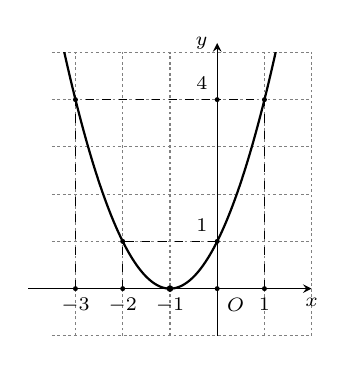
\begin{tikzpicture}[>=stealth,x=1cm,y=1cm,scale=0.6]
					\def\a{1} % Hệ số a phải khác 0
					\def\b{2}
					\def\c{1}
					\draw[color=gray,dash pattern=on 1pt off 1pt,xstep=1.0cm,ystep=1.0cm] (-3.5,-1) grid (2,5);
					\draw[->] (-4,0) -- (2,0) node[below] {\scriptsize $x$};
					\draw[->] (0,-1) -- (0,5.2) node[left] {\scriptsize $y$};
					\draw[dashed] (0,0)node[below right]{\scriptsize $O$} (-3, 0) node[below]{\scriptsize $-3$}--(-3,4)--(0, 4) node[above left]{\scriptsize $4$} (-2, 0) node[below]{\scriptsize $-2$}--(-2,1)--(0, 1) node[above left]{\scriptsize $1$} (-1, 0)node[below]{\scriptsize $-1$} (1, 0) node[below]{\scriptsize $1$}--(1,4)--(0, 4) ;
					\pgfmathsetmacro\xdinh{-(\b)/2*(\a)}
					\pgfmathsetmacro\ydinh{(4*(\a)*(\c)-(\b)^2)/(4*(\a))}
					\fill[dashed] (\xdinh,\ydinh)circle(2pt) edge (\xdinh,0) edge (0,\ydinh);
					\clip (-3.5,-1)rectangle(2,5);
					\draw[thick,samples=150,smooth,domain=-3.5:1.5] plot(\x,{\a*(\x)^2+(\b)*\x+(\c)});
					\foreach \x/\y in{0/0, -3/0, -3/4, -2/0, -2/1, 0/1, 1/0, 1/4, 0/4}
					\fill[black](\x,\y) circle (1.5pt);
			\end{tikzpicture}}
			\item 
			\immini{Ta có $a=-1, b=2, c=-2, \Delta =(2)^2-4\cdot (-1)\cdot (-2)=-4$.
				\begin{itemize}
					\item Tọa độ đỉnh $I\left(1;-1\right)$.
					\item Trục đối xứng $x=1$.
					\item Bảng giá trị
					\begin{center}
						\begin{tabular}{|c|c|c|c|c|c|}
							\hline
							$x$	&$-1$ &$0$ &$1$ &$2$ &$3$ \\
							\hline
							$y$	& $-5$ & $-2$ & $-1$ & $-2$ &$-5$ \\
							\hline
						\end{tabular}	
					\end{center}
				\end{itemize}
				Vẽ parabol đi qua các điểm được xác định ở trên, ta nhận được đồ thị hàm số $y=-x^2+2x-2$.}{	
				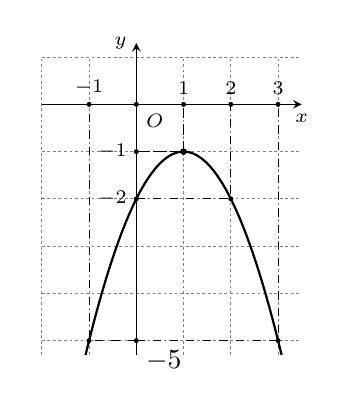
\begin{tikzpicture}[>=stealth,x=1cm,y=1cm,scale=0.6]
					\def\a{-1} % Hệ số a phải khác 0
					\def\b{2}
					\def\c{-2}
					\draw[color=gray,dash pattern=on 1pt off 1pt,xstep=1.0cm,ystep=1.0cm] (-2,-5.3) grid (3.5,1);
					\draw[->] (-2,0) -- (3.5,0) node[below] {\scriptsize $x$};
					\draw[->] (0,-5.3) -- (0,1.3) node[left] {\scriptsize $y$};
					\draw[dashed] (0,0)node[below right]{\scriptsize $O$} (0, -5)node[below right]{$\scriptsize -5$}--(-1, -5)--(-1, 0)node[above]{\scriptsize $-1$} (0, -1)node[left]{\scriptsize $-1$}--(1, -1)--(1, 0)node[above]{\scriptsize $1$} (0, -2)node[left]{\scriptsize $-2$}--(2, -2)--(2, 0)node[above]{\scriptsize $2$} (0, -5)--(3, -5)--(3, 0)node[above]{\scriptsize $3$};
					\pgfmathsetmacro\xdinh{-(\b)/2*(\a)}
					\pgfmathsetmacro\ydinh{(4*(\a)*(\c)-(\b)^2)/(4*(\a))}
					\fill[dashed] (\xdinh,\ydinh)circle(2pt) edge (\xdinh,0) edge (0,\ydinh);
					\clip (-2.3,-5.3)rectangle(3.3,1);
					\draw[thick,samples=150,smooth,domain=-2.3:3.3] plot(\x,{\a*(\x)^2+(\b)*\x+(\c)});
					\foreach \x/\y in{0/0,0/-5, 0/-2, -1/0, 2/0, 3/0, 3/-5, -1/-5, 0/-1, 2/-2, 1/0}
					\fill[black](\x,\y) circle (1.5pt);
			\end{tikzpicture}}
		\end{enumEX}
	}	
\end{bt}

% nguồn: chuyen_dang (nhập 22/11/2026)
\begin{ex}%[1C2H1-2]%[ma:1628c02e]
	Tìm đạo hàm cấp hai của các hàm số  sau:
	\begin{enumEX}{4}
		\item $y=\dfrac{1}{1-x}$, 
		\item  $y=\dfrac{1}{\sqrt{1-x}}$,
		\item $y=\tan  x$,
		 \item $y=\cos^2x$.
	\end{enumEX}
	 \loigiai{
		\begin{enumerate}
			 \item Ta có $y'=\dfrac{1}{(1-x)^2}$ và $y''=\dfrac{2}{(1-x)^3}$.
			\item Ta có $y'=\dfrac{1}{2(1-x)\sqrt{1-x}}$ và $y''=\dfrac{3}{4(1-x)^2\sqrt{1-x}}$. 
			\item Ta có $y'=\dfrac{1}{\cos^2x}$  và $y''=\dfrac{2\sin x}{\cos^3x}$.
			\item Ta có $y=\dfrac{1}{2}+\dfrac{1}{2}\cos 2x$. Khi đó $y'=-\sin 2x$ và $y''=-2\cos  2x$.
		\end{enumerate}
	 }
\end{ex}

% nguồn: chuyen_dang (nhập 22/11/2026)
\begin{bt}%[1C2N1-2]%[ma:f81eb590]
% nguon: Archive/2024/SP-K10-K11-LyVanHoang_TVN-023/11. C1-LuongGiac-lvhoang_TVN-023/dataC1K11/Bai2-Dang1-Congthuccong.tex #1924
%[Cánh Diều]%[Đỗ Vũ Minh Thắng, 24-25 BG 10 11]
	Tính
	\begin{enumEX}{2}
		\item $\tan \dfrac{7 \pi}{12}$.
		\item $\tan 165^{\circ}$.
	\end{enumEX}
	\loigiai{
		\begin{listEX}[1]
			\item Áp dụng công thức cộng đối với tang, ta có\\
			$\tan \dfrac{7 \pi}{12}=\tan \left(\dfrac{\pi}{4}+\dfrac{\pi}{3}\right)=\dfrac{\tan \frac{\pi}{4}+\tan \frac{\pi}{3}}{1-\tan \frac{\pi}{4} \tan \frac{\pi}{3}}=\dfrac{1+\sqrt{3}}{1-\sqrt{3}}=-2-\sqrt{3}$.
			\item Áp dụng công thức cộng đối với tang, ta có\\
			$\tan 15^{\circ}=\tan \left(45^{\circ}-30^{\circ}\right)=\dfrac{\tan 45^{\circ}-\tan 30^{\circ}}{1+\tan 45^{\circ} \tan 30^{\circ}}=\dfrac{1-\frac{\sqrt{3}}{3}}{1+\frac{\sqrt{3}}{3}}=2-\sqrt{3}$.
		\end{listEX}
	}
\end{bt}

% nguồn: chuyen_dang (nhập 22/11/2026)
\begin{bt}%[1C2H1-2]%[ma:c20b68c5]
	Tìm các khoảng đồng biến, nghịch biến  và các điểm cực trị của các hàm số sau:
	\begin{enumEX}{2}
		 \item $y=2x^3+3x^2-12x+2\,024$.
		 \item $y=x^4+2\,024$.
		\item $y=-\dfrac{1}{4}x^4+2x^2+2$. 
		\item $y=x^4-2x^2-2$. 
	\end{enumEX}
	\loigiai{ 
		\begin{enumEX}{1}
			 \item
			Ta có: $y'=6x^2+6x-12=0 \Leftrightarrow\hoac{&x=1  \\ &x=-2.}$\\
			Bảng biến  thiên:
			\begin{center}
				\begin{tikzpicture}
					\tkzTabInit[lgt=1.2,espcl=2.5] 
						{$x$ /0.8,$f’(x)$ /0.8,$f (x)$ /2.5} 
						{$-\infty$,$-2$,$1$,$+\infty$} 
					 \tkzTabLine{,+,0,-,0,+,}
					 \tkzTabVar{-/$-\infty$,+/$2\,044$,-/$2\,017$,+/$+\infty$}
				\end{tikzpicture}
			\end{center}
			 Quan sát bảng biến thiên ta có hàm số đồng biến trên các khoảng $(-\infty;-2)$, $(1;+\infty)$ và nghịch biến trên khoảng $(-2; 1)$.\\
			Hàm số đạt cực  đại tại điểm $x=-2$, giá trị cực đại $y=2044$.\\
			Hàm số đạt  cực tiểu tại điểm $x=1$, giá trị cực tiểu $y=2017$.
			 \item Ta có tập xác định $D=\mathbb{R}$ và có đạo hàm $y'=4x^3$; $y'=0 \Leftrightarrow 4x^3=0 \Leftrightarrow x=0$.\\
			Bảng  biến thiên
			\begin{center}
				\begin{tikzpicture}
					\tkzTabInit[lgt=1.2,espcl=3.5] 
						{$x$/0.8,$f’(x)$/0.8,$f  (x)$/2.5}
						 {$-\infty$,$0$,$+\infty$}
					 \tkzTabLine{,-,0,+,}
					 \tkzTabVar{+/$+\infty$,-/$2\,024$,+/$+\infty$}
				\end{tikzpicture}
			\end{center}
			Từ bảng biến thiên, hàm số đồng biến  trên khoảng $(0;+\infty)$ và nghịch biến trên khoảng $(-\infty; 0)$.\\
			Hàm số đạt cực tiểu tại điểm $x=0$, giá trị cực tiểu $y=2\,024$. 
			 \item Tập xác định $D=\mathbb{R}$.\\
			Đạo hàm $y'=-x^3+4x=-x(x^2-4)$; $y'=0 \Leftrightarrow-x(x^2-4)=0 \Leftrightarrow\hoac{&x=0 \\& x= \pm  2.}$\\
			Bảng  biến thiên
			\begin{center}
				\begin{tikzpicture}
					 \tkzTabInit[lgt=1.2,espcl=2.5]
						 {$x$/0.8,$f’(x)$/0.8,$f (x)$/2.5}
						 {$-\infty$,$-2$,$0$,$2$,$+\infty$}
					\tkzTabLine{,+,0,-,0,+,0,-,} 
					\tkzTabVar{-/$-\infty$,+/$6$,-/$2$,+/$6$,-/$-\infty$} 
				\end{tikzpicture}
			\end{center}
			 Suy ra hàm số nghịch biến trên các khoảng $(-2;0)$ và $(2;+\infty)$, đồng biến trên các khoảng $(0;2)$ và $(-\infty;-2)$.\\
			Hàm số đạt cực đại tại điểm $x=  \pm 2$, giá trị cực đại $y=6$.\\
			Hàm số đạt cực tiểu tại  điểm $x=0$, giá trị cực tiểu $y=2$.
			\item Tập  xác định $D=\mathbb{R}$.\\
			Ta có $y'=4x^3-4x$, $y'=0 \Leftrightarrow  x=0, x= \pm 1$.\\
			Bảng  biến thiên
			\begin{center}
				\begin{tikzpicture}
					\tkzTabInit[lgt=1.2,espcl=2.5] 
						{$x$/0.8,$f’(x)$/0.8,$f (x)$/2.5} 
						 {$-\infty$,$-1$,$0$,$1$,$+\infty$}
					\tkzTabLine{,-,0,+,0,-,0,+,} 
					\tkzTabVar{+/$+\infty$,-/$-3$,+/$-2$,-/$-3$,+/$+\infty$} 
				\end{tikzpicture}
			\end{center}
			Từ bảng  biến thiên ta suy ra hàm số nghịch biến trên mỗi khoảng $(-\infty;-1)$ và $(0; 1)$ và đồng biến trên các khoảng $(-1;0)$, $(1;+\infty)$.\\
			Hàm số đạt cực đại tại điểm $x=0$, giá trị  cực đại $y=-2$.\\
			Hàm số đạt cực tiểu  tại điểm $x= \pm 1$, giá trị cực tiểu $y=-3$.
		\end{enumEX}
	} 
\end{bt}

% nguồn: chuyen_dang (nhập 22/11/2026)
\begin{bt}%[1C2Y1-2]%[ma:7475a090]
	Viết năm số hạng đầu và số hạng thứ 100 của các dãy số $(u_n)$ có số  hạng tổng quát cho bởi:
	\begin{enumEX}[a)]{3}
		\item  $u_n=3 n-2$;
		\item $u_n=3 \cdot 2^n$; 
		\item  $u_n=\left(1+\dfrac{1}{n}\right)^{n}$.
	\end{enumEX}
	 \loigiai{
		\begin{enumEX}[a)]{1}
			\item $u_1=3\cdot 1-2=1;$ $u_2=3\cdot 2-2=4;$ $u_3=3\cdot 3-2=7;$  $u_4=3\cdot 4-2=10;$ $u_5=3\cdot 5-2=13;$ $u_{100}=3\cdot 100-2=298.$
			\item $u_1=3 \cdot 2^1=6;$ $u_2=3 \cdot 2^2=12;$ $u_3=3 \cdot 2^3=24;$ $u_4=3 \cdot 2^4=48;$ $u_5=3 \cdot 2^5=96;$  $u_{100}=3 \cdot 2^{100}.$
			\item $u_1=\left(1+\dfrac{1}{1}\right)^{1}=2$; $u_2=\left(1+\dfrac{1}{2}\right)^{2}=\dfrac{9}{4}$; $u_3=\left(1+\dfrac{1}{3}\right)^{3}=\dfrac{64}{27}$; $u_4=\left(1+\dfrac{1}{4}\right)^{4}=\dfrac{625}{256}$; $u_5=\left(1+\dfrac{1}{5}\right)^{5}=\dfrac{1296}{625}$;  $u_{100}=\left(1+\dfrac{1}{100}\right)^{100}$.
	\end{enumEX}}
\end{bt}

% nguồn: chuyen_dang (nhập 22/11/2026)
\begin{bt}%[1C2H1-2]%[ma:61a11692]
	Tìm các khoảng đồng biến, nghịch biến của các hàm  số sau:
	\begin{enumEX}{2}
		\item  $y=\sqrt{x^2-6x+5}$.
		\item  $y=\dfrac{5x+9}{x-1}$.
		 \item $y=(x-2)\left(x^2+1\right)$.
		\item  $y=\dfrac{x^2+2x+2}{x+1}$.
	\end{enumEX}
	 \loigiai{
		\begin{enumEX}{1}
			\item Tập xác định  $ \mathscr{D}= (-\infty;1]\cup [5;+\infty)$.\\
			Ta có $ y' = \dfrac{x - 3}{\sqrt{x^2 - 6x + 5}} $; $y'=0\Leftrightarrow x-3=0\Leftrightarrow  x=3\notin \mathscr{D}$. Ta có bảng biến thiên
			\begin{center}
				
\begin{tikzpicture}[scale=1]
					\tikzset{h style/.style  ={pattern=north west lines}}
					\tkzTabInit[lgt=1.5,espcl=2.5]{$x$ /1,$y'$  /1,$y$ /2}
						{$-\infty$,$ 1 $,$ 5 $,$+\infty$} 
					\tkzTabLine{,-,d,h,d,+,} 
					\tkzTabVar{+/$+\infty$,-H/$0$,-/$0$,+/$+\infty  $}
				\end{tikzpicture}
			\end{center}
			Ta thấy hàm số đồng  biến trên $ (5; + \infty) $.
			 \item Tập xác định của hàm số $\mathscr{D}=\mathbb{R}\setminus\{1\}$.\\
			Do $y'=\dfrac{(5x+9)'(x-1)-(x-1)'(5x+9)}{(x-1)^2}=-\dfrac{14}{(x-1)^2}<0,\,\forall x\in\mathscr{D}$ suy ra hàm số nghịch biến  trên các khoảng $(-\infty;1)$ và $(1,+\infty)$.
			\item Ta có $y=x^3-2x^2+x-2$, tập xác định $\mathscr{D}=\mathbb{R}$. Đạo  hàm
			$y'=3x^2-4x+1$.\\ 
			Giải phương trình $y'=0  \Leftrightarrow \hoac{&x=1\\&x=\dfrac{1}{3}.}$\\
			Ta có bảng xét dấu  của đạo hàm.
			\begin{center}
				
\begin{tikzpicture}[>=stealth,scale=1]
					\tkzTabInit[nocadre=false,lgt=1.2,espcl=2.5,deltacl=0.6] 
						{$x$ /1,$y’$ /0.8} 
						 {$-\infty$,$\dfrac{1}{3}$,$1$,$+\infty$}
					 \tkzTabLine{,+,z,-,z,+,}
				\end{tikzpicture}
			\end{center}
			Từ bảng xét dấu đạo hàm ta thấy hàm số  nghịch biến trên khoảng $\left(\dfrac{1}{3};1\right)$ và đồng biến trên các khoảng $\left(-\infty;\dfrac{1}{3}\right)$ và $(1;+\infty)$.
			\item \begin{itemize}
			\item Tập xác định  $\mathscr{D}=\mathbb{R}\setminus \left\{-1\right\}$.
			\item $y'=\dfrac{x^2+2x}{(x+1)^2}$, $y'=0\Leftrightarrow \hoac{&  x=-2 \\ & x=0.}$\\
			Ta có  bảng biến thiên
			\begin{center}
				
\begin{tikzpicture}
					\tkzTabInit[nocadre=false,lgt=1,espcl=2] 
						 {$x$ /0.7,$y'$ /0.7,$y$ /2}
						 {$-\infty$,$-2$,$-1$,$0$,$+\infty$}
					\tkzTabLine{,+,$0$,-,d,-,$0$,+,} 
					\tkzTabVar{-/$-\infty$,+/$-2$,-D+/$-\infty$/$+\infty$,-/$2$,+/$+\infty$} 
				\end{tikzpicture}
			\end{center}
			Hàm số đồng biến trên khoảng  $\left( -\infty;-2\right)$ và $\left( 0;+\infty\right)$; nghịch biến trên $(-2;-1)$ và $(-1;0)$.
		\end{itemize}
	\end{enumEX}
 }
\end{bt}
